\documentclass[a4paper]{article}
\usepackage{makeidx}
\usepackage{natbib}
\usepackage{graphicx}
\usepackage{multicol}
\usepackage{float}
\usepackage{listings}
\usepackage{color}
\usepackage{ifthen}
\usepackage[table]{xcolor}
\usepackage{textcomp}
\usepackage{alltt}
\usepackage{ifpdf}
\ifpdf
\usepackage[pdftex,
            pagebackref=true,
            colorlinks=true,
            linkcolor=blue,
            unicode
           ]{hyperref}
\else
\usepackage[ps2pdf,
            pagebackref=true,
            colorlinks=true,
            linkcolor=blue,
            unicode
           ]{hyperref}
\usepackage{pspicture}
\fi
\usepackage[utf8]{inputenc}
\usepackage{mathptmx}
\usepackage[scaled=.90]{helvet}
\usepackage{courier}
\usepackage{sectsty}
\usepackage[titles]{tocloft}
\usepackage{doxygen}
\lstset{language=C++,inputencoding=utf8,basicstyle=\footnotesize,breaklines=true,breakatwhitespace=true,tabsize=8,numbers=left }
\makeindex
\setcounter{tocdepth}{3}
\renewcommand{\footrulewidth}{0.4pt}
\renewcommand{\familydefault}{\sfdefault}
\hfuzz=15pt
\setlength{\emergencystretch}{15pt}
\hbadness=750
\tolerance=750
\begin{document}
\hypersetup{pageanchor=false,citecolor=blue}
\begin{titlepage}
\vspace*{7cm}
\begin{center}
{\Large \-Notatio \-Antiqua \\[1ex]\large 1.\-0.\-0.\-3164pre }\\
\vspace*{1cm}
{\large \-Generated by Doxygen 1.7.6.1}\\
\vspace*{0.5cm}
{\small Tue Jun 12 2012 17:27:11}\\
\end{center}
\end{titlepage}
\pagenumbering{roman}
\tableofcontents
\pagenumbering{arabic}
\hypersetup{pageanchor=true,citecolor=blue}
\section{\-Notatio \-Antiqua}
\label{index}\hypertarget{index}{}\chapter{Notatio Antiqua}
\hypertarget{index}{}\label{index}\index{Notatio Antiqua@{Notatio Antiqua}}
Notatio Antiqua is an Open Source GUI for creating PDFs with gregorio and Lua\+La\+TeX at the moment it is in beta testing phase, not everything will function as expected 
\section{\-Namespace \-Index}
\input{namespaces}
\section{\-Class \-Index}
\doxysection{Class List}
Here are the classes, structs, unions and interfaces with brief descriptions\+:\begin{DoxyCompactList}
\item\contentsline{section}{\mbox{\hyperlink{struct___hash_entry}{\+\_\+\+Hash\+Entry}} }{\pageref{struct___hash_entry}}{}
\item\contentsline{section}{\mbox{\hyperlink{struct___hash_tab}{\+\_\+\+Hash\+Tab}} }{\pageref{struct___hash_tab}}{}
\item\contentsline{section}{\mbox{\hyperlink{struct___hyphen_dict}{\+\_\+\+Hyphen\+Dict}} }{\pageref{struct___hyphen_dict}}{}
\item\contentsline{section}{\mbox{\hyperlink{struct___hyphen_state}{\+\_\+\+Hyphen\+State}} }{\pageref{struct___hyphen_state}}{}
\item\contentsline{section}{\mbox{\hyperlink{struct___hyphen_trans}{\+\_\+\+Hyphen\+Trans}} }{\pageref{struct___hyphen_trans}}{}
\item\contentsline{section}{\mbox{\hyperlink{class_highlighter}{Highlighter}} \\*\mbox{[}0\mbox{]} }{\pageref{class_highlighter}}{}
\item\contentsline{section}{\mbox{\hyperlink{class_mdi_child}{Mdi\+Child}} }{\pageref{class_mdi_child}}{}
\item\contentsline{section}{\mbox{\hyperlink{classnaapplication}{naapplication}} }{\pageref{classnaapplication}}{}
\item\contentsline{section}{\mbox{\hyperlink{class_n_a_clef_select}{NAClef\+Select}} }{\pageref{class_n_a_clef_select}}{}
\item\contentsline{section}{\mbox{\hyperlink{classnadoinit}{nadoinit}} }{\pageref{classnadoinit}}{}
\item\contentsline{section}{\mbox{\hyperlink{classnafindreplace}{nafindreplace}} }{\pageref{classnafindreplace}}{}
\item\contentsline{section}{\mbox{\hyperlink{class_n_a_header_wizard}{NAHeader\+Wizard}} }{\pageref{class_n_a_header_wizard}}{}
\item\contentsline{section}{\mbox{\hyperlink{class_n_a_help}{NAHelp}} }{\pageref{class_n_a_help}}{}
\item\contentsline{section}{\mbox{\hyperlink{classnainit}{nainit}} }{\pageref{classnainit}}{}
\item\contentsline{section}{\mbox{\hyperlink{classnajgabc}{najgabc}} }{\pageref{classnajgabc}}{}
\item\contentsline{section}{\mbox{\hyperlink{class_na_prog}{Na\+Prog}} }{\pageref{class_na_prog}}{}
\item\contentsline{section}{\mbox{\hyperlink{classnapsalm}{napsalm}} \\*Class for holding the information on psalm tone models }{\pageref{classnapsalm}}{}
\item\contentsline{section}{\mbox{\hyperlink{class_n_a_settings}{NASettings}} \\*Settings class, holds some variables for the settings dialog and the dialog itself }{\pageref{class_n_a_settings}}{}
\item\contentsline{section}{\mbox{\hyperlink{struct_q_header_info}{QHeader\+Info}} }{\pageref{struct_q_header_info}}{}
\item\contentsline{section}{\mbox{\hyperlink{class_q_help_browser}{QHelp\+Browser}} }{\pageref{class_q_help_browser}}{}
\end{DoxyCompactList}

\section{\-File \-Index}
\subsection{\-File \-List}
\-Here is a list of all files with brief descriptions\-:\begin{DoxyCompactList}
\item\contentsline{section}{\hyperlink{hnjalloc_8c}{hnjalloc.\-c} }{\pageref{hnjalloc_8c}}{}
\item\contentsline{section}{\hyperlink{hnjalloc_8h}{hnjalloc.\-h} }{\pageref{hnjalloc_8h}}{}
\item\contentsline{section}{\hyperlink{hyphen_8c}{hyphen.\-c} }{\pageref{hyphen_8c}}{}
\item\contentsline{section}{\hyperlink{hyphen_8h}{hyphen.\-h} }{\pageref{hyphen_8h}}{}
\item\contentsline{section}{\hyperlink{main_8cpp}{main.\-cpp} }{\pageref{main_8cpp}}{}
\item\contentsline{section}{\hyperlink{naapplication_8cpp}{naapplication.\-cpp} }{\pageref{naapplication_8cpp}}{}
\item\contentsline{section}{\hyperlink{naapplication_8h}{naapplication.\-h} }{\pageref{naapplication_8h}}{}
\item\contentsline{section}{\hyperlink{naclefselect_8cpp}{naclefselect.\-cpp} }{\pageref{naclefselect_8cpp}}{}
\item\contentsline{section}{\hyperlink{naclefselect_8h}{naclefselect.\-h} }{\pageref{naclefselect_8h}}{}
\item\contentsline{section}{\hyperlink{nadoinit_8cpp}{nadoinit.\-cpp} }{\pageref{nadoinit_8cpp}}{}
\item\contentsline{section}{\hyperlink{nadoinit_8h}{nadoinit.\-h} }{\pageref{nadoinit_8h}}{}
\item\contentsline{section}{\hyperlink{naheaderwizard_8cpp}{naheaderwizard.\-cpp} }{\pageref{naheaderwizard_8cpp}}{}
\item\contentsline{section}{\hyperlink{naheaderwizard_8h}{naheaderwizard.\-h} }{\pageref{naheaderwizard_8h}}{}
\item\contentsline{section}{\hyperlink{nahelp_8cpp}{nahelp.\-cpp} }{\pageref{nahelp_8cpp}}{}
\item\contentsline{section}{\hyperlink{nahelp_8h}{nahelp.\-h} }{\pageref{nahelp_8h}}{}
\item\contentsline{section}{\hyperlink{nainit_8cpp}{nainit.\-cpp} }{\pageref{nainit_8cpp}}{}
\item\contentsline{section}{\hyperlink{nainit_8h}{nainit.\-h} }{\pageref{nainit_8h}}{}
\item\contentsline{section}{\hyperlink{namdi_8cpp}{namdi.\-cpp} }{\pageref{namdi_8cpp}}{}
\item\contentsline{section}{\hyperlink{namdi_8h}{namdi.\-h} }{\pageref{namdi_8h}}{}
\item\contentsline{section}{\hyperlink{naprog_8cpp}{naprog.\-cpp} }{\pageref{naprog_8cpp}}{}
\item\contentsline{section}{\hyperlink{naprog_8h}{naprog.\-h} }{\pageref{naprog_8h}}{}
\item\contentsline{section}{\hyperlink{napsalm_8cpp}{napsalm.\-cpp} }{\pageref{napsalm_8cpp}}{}
\item\contentsline{section}{\hyperlink{napsalm_8h}{napsalm.\-h} }{\pageref{napsalm_8h}}{}
\item\contentsline{section}{\hyperlink{nasettings_8cpp}{nasettings.\-cpp} }{\pageref{nasettings_8cpp}}{}
\item\contentsline{section}{\hyperlink{nasettings_8h}{nasettings.\-h} }{\pageref{nasettings_8h}}{}
\item\contentsline{section}{\hyperlink{nasyntax_8cpp}{nasyntax.\-cpp} }{\pageref{nasyntax_8cpp}}{}
\item\contentsline{section}{\hyperlink{nasyntax_8h}{nasyntax.\-h} }{\pageref{nasyntax_8h}}{}
\item\contentsline{section}{\hyperlink{naview_8cpp}{naview.\-cpp} }{\pageref{naview_8cpp}}{}
\item\contentsline{section}{\hyperlink{naview_8h}{naview.\-h} }{\pageref{naview_8h}}{}
\item\contentsline{section}{\hyperlink{version_8h}{version.\-h} }{\pageref{version_8h}}{}
\end{DoxyCompactList}

\section{\-Namespace \-Documentation}
\hypertarget{namespace_ui}{\subsection{\-Ui \-Namespace \-Reference}
\label{namespace_ui}\index{\-Ui@{\-Ui}}
}

\input{namespace_version}
\section{\-Class \-Documentation}
\hypertarget{struct___hash_entry}{\subsection{\-\_\-\-Hash\-Entry \-Struct \-Reference}
\label{struct___hash_entry}\index{\-\_\-\-Hash\-Entry@{\-\_\-\-Hash\-Entry}}
}
\subsubsection*{\-Public \-Attributes}
\begin{DoxyCompactItemize}
\item 
\hyperlink{hyphen_8c_a5ee9ebda39a0bc28128d176a5018151c}{\-Hash\-Entry} $\ast$ \hyperlink{struct___hash_entry_acd1ec10363520d8cf32205e03e3e3493}{next}
\item 
char $\ast$ \hyperlink{struct___hash_entry_a00e4de3cd14f3263e8505e2e3e77c605}{key}
\item 
int \hyperlink{struct___hash_entry_a1acd8c25274e1385e1d0624f398e2a06}{val}
\end{DoxyCompactItemize}


\subsubsection{\-Detailed \-Description}


\-Definition at line 98 of file hyphen.\-c.



\subsubsection{\-Member \-Data \-Documentation}
\hypertarget{struct___hash_entry_a00e4de3cd14f3263e8505e2e3e77c605}{\index{\-\_\-\-Hash\-Entry@{\-\_\-\-Hash\-Entry}!key@{key}}
\index{key@{key}!_HashEntry@{\-\_\-\-Hash\-Entry}}
\paragraph[{key}]{\setlength{\rightskip}{0pt plus 5cm}char$\ast$ {\bf \-\_\-\-Hash\-Entry\-::key}}}\label{struct___hash_entry_a00e4de3cd14f3263e8505e2e3e77c605}


\-Definition at line 100 of file hyphen.\-c.

\hypertarget{struct___hash_entry_acd1ec10363520d8cf32205e03e3e3493}{\index{\-\_\-\-Hash\-Entry@{\-\_\-\-Hash\-Entry}!next@{next}}
\index{next@{next}!_HashEntry@{\-\_\-\-Hash\-Entry}}
\paragraph[{next}]{\setlength{\rightskip}{0pt plus 5cm}{\bf \-Hash\-Entry}$\ast$ {\bf \-\_\-\-Hash\-Entry\-::next}}}\label{struct___hash_entry_acd1ec10363520d8cf32205e03e3e3493}


\-Definition at line 99 of file hyphen.\-c.

\hypertarget{struct___hash_entry_a1acd8c25274e1385e1d0624f398e2a06}{\index{\-\_\-\-Hash\-Entry@{\-\_\-\-Hash\-Entry}!val@{val}}
\index{val@{val}!_HashEntry@{\-\_\-\-Hash\-Entry}}
\paragraph[{val}]{\setlength{\rightskip}{0pt plus 5cm}int {\bf \-\_\-\-Hash\-Entry\-::val}}}\label{struct___hash_entry_a1acd8c25274e1385e1d0624f398e2a06}


\-Definition at line 101 of file hyphen.\-c.



\-The documentation for this struct was generated from the following file\-:\begin{DoxyCompactItemize}
\item 
\hyperlink{hyphen_8c}{hyphen.\-c}\end{DoxyCompactItemize}

\hypertarget{struct___hash_tab}{\subsection{\-\_\-\-Hash\-Tab \-Struct \-Reference}
\label{struct___hash_tab}\index{\-\_\-\-Hash\-Tab@{\-\_\-\-Hash\-Tab}}
}
\subsubsection*{\-Public \-Attributes}
\begin{DoxyCompactItemize}
\item 
\hyperlink{hyphen_8c_a5ee9ebda39a0bc28128d176a5018151c}{\-Hash\-Entry} $\ast$ \hyperlink{struct___hash_tab_ac846f490560903e5d82191d1f45e7ae3}{entries} \mbox{[}\hyperlink{hyphen_8c_ad6074dd11ab3c97c8135c43aab03ae95}{\-H\-A\-S\-H\-\_\-\-S\-I\-Z\-E}\mbox{]}
\end{DoxyCompactItemize}


\subsubsection{\-Detailed \-Description}


\-Definition at line 94 of file hyphen.\-c.



\subsubsection{\-Member \-Data \-Documentation}
\hypertarget{struct___hash_tab_ac846f490560903e5d82191d1f45e7ae3}{\index{\-\_\-\-Hash\-Tab@{\-\_\-\-Hash\-Tab}!entries@{entries}}
\index{entries@{entries}!_HashTab@{\-\_\-\-Hash\-Tab}}
\paragraph[{entries}]{\setlength{\rightskip}{0pt plus 5cm}{\bf \-Hash\-Entry}$\ast$ {\bf \-\_\-\-Hash\-Tab\-::entries}\mbox{[}{\bf \-H\-A\-S\-H\-\_\-\-S\-I\-Z\-E}\mbox{]}}}\label{struct___hash_tab_ac846f490560903e5d82191d1f45e7ae3}


\-Definition at line 95 of file hyphen.\-c.



\-The documentation for this struct was generated from the following file\-:\begin{DoxyCompactItemize}
\item 
\hyperlink{hyphen_8c}{hyphen.\-c}\end{DoxyCompactItemize}

\hypertarget{struct___hyphen_dict}{\subsection{\-\_\-\-Hyphen\-Dict \-Struct \-Reference}
\label{struct___hyphen_dict}\index{\-\_\-\-Hyphen\-Dict@{\-\_\-\-Hyphen\-Dict}}
}


{\ttfamily \#include $<$hyphen.\-h$>$}

\subsubsection*{\-Public \-Attributes}
\begin{DoxyCompactItemize}
\item 
char \hyperlink{struct___hyphen_dict_abadeccbce027b36645841686ad93d067}{lhmin}
\item 
char \hyperlink{struct___hyphen_dict_a3440b9768543e97e7e80d4ba29e1fa75}{rhmin}
\item 
char \hyperlink{struct___hyphen_dict_a651eac97882c11ba2416f21ab8a4ed79}{clhmin}
\item 
char \hyperlink{struct___hyphen_dict_a32f506e9ca1f4746acb0c41b33887e80}{crhmin}
\item 
char $\ast$ \hyperlink{struct___hyphen_dict_aca2a1b71c4669b45d9ae7ec1377dda2d}{nohyphen}
\item 
int \hyperlink{struct___hyphen_dict_a581693f2d9c912e4388759fae8623ef1}{nohyphenl}
\item 
int \hyperlink{struct___hyphen_dict_a82c9b7aefbd4dcec7302a9bbc2247acc}{num\-\_\-states}
\item 
char \hyperlink{struct___hyphen_dict_a53f12e09d8005867c7cbcc91a88befea}{cset} \mbox{[}\hyperlink{hyphen_8h_ac7c0207aa5a0e10d378be03b68041350}{\-M\-A\-X\-\_\-\-N\-A\-M\-E}\mbox{]}
\item 
int \hyperlink{struct___hyphen_dict_afd01aac8b36d018ec931891e0e95a570}{utf8}
\item 
\hyperlink{hyphen_8h_a633ccfbecf941f82b956182be6ffb59b}{\-Hyphen\-State} $\ast$ \hyperlink{struct___hyphen_dict_a27a77f586dc0a6925d074ba61294d985}{states}
\item 
\hyperlink{hyphen_8h_aa4f1bc9b13f797026fc4e49b8ea7928a}{\-Hyphen\-Dict} $\ast$ \hyperlink{struct___hyphen_dict_a6fb0dc613da914a03c2e09e0483246be}{nextlevel}
\end{DoxyCompactItemize}


\subsubsection{\-Detailed \-Description}


\-Definition at line 64 of file hyphen.\-h.



\subsubsection{\-Member \-Data \-Documentation}
\hypertarget{struct___hyphen_dict_a651eac97882c11ba2416f21ab8a4ed79}{\index{\-\_\-\-Hyphen\-Dict@{\-\_\-\-Hyphen\-Dict}!clhmin@{clhmin}}
\index{clhmin@{clhmin}!_HyphenDict@{\-\_\-\-Hyphen\-Dict}}
\paragraph[{clhmin}]{\setlength{\rightskip}{0pt plus 5cm}char {\bf \-\_\-\-Hyphen\-Dict\-::clhmin}}}\label{struct___hyphen_dict_a651eac97882c11ba2416f21ab8a4ed79}


\-Definition at line 68 of file hyphen.\-h.

\hypertarget{struct___hyphen_dict_a32f506e9ca1f4746acb0c41b33887e80}{\index{\-\_\-\-Hyphen\-Dict@{\-\_\-\-Hyphen\-Dict}!crhmin@{crhmin}}
\index{crhmin@{crhmin}!_HyphenDict@{\-\_\-\-Hyphen\-Dict}}
\paragraph[{crhmin}]{\setlength{\rightskip}{0pt plus 5cm}char {\bf \-\_\-\-Hyphen\-Dict\-::crhmin}}}\label{struct___hyphen_dict_a32f506e9ca1f4746acb0c41b33887e80}


\-Definition at line 69 of file hyphen.\-h.

\hypertarget{struct___hyphen_dict_a53f12e09d8005867c7cbcc91a88befea}{\index{\-\_\-\-Hyphen\-Dict@{\-\_\-\-Hyphen\-Dict}!cset@{cset}}
\index{cset@{cset}!_HyphenDict@{\-\_\-\-Hyphen\-Dict}}
\paragraph[{cset}]{\setlength{\rightskip}{0pt plus 5cm}char {\bf \-\_\-\-Hyphen\-Dict\-::cset}\mbox{[}{\bf \-M\-A\-X\-\_\-\-N\-A\-M\-E}\mbox{]}}}\label{struct___hyphen_dict_a53f12e09d8005867c7cbcc91a88befea}


\-Definition at line 75 of file hyphen.\-h.

\hypertarget{struct___hyphen_dict_abadeccbce027b36645841686ad93d067}{\index{\-\_\-\-Hyphen\-Dict@{\-\_\-\-Hyphen\-Dict}!lhmin@{lhmin}}
\index{lhmin@{lhmin}!_HyphenDict@{\-\_\-\-Hyphen\-Dict}}
\paragraph[{lhmin}]{\setlength{\rightskip}{0pt plus 5cm}char {\bf \-\_\-\-Hyphen\-Dict\-::lhmin}}}\label{struct___hyphen_dict_abadeccbce027b36645841686ad93d067}


\-Definition at line 66 of file hyphen.\-h.

\hypertarget{struct___hyphen_dict_a6fb0dc613da914a03c2e09e0483246be}{\index{\-\_\-\-Hyphen\-Dict@{\-\_\-\-Hyphen\-Dict}!nextlevel@{nextlevel}}
\index{nextlevel@{nextlevel}!_HyphenDict@{\-\_\-\-Hyphen\-Dict}}
\paragraph[{nextlevel}]{\setlength{\rightskip}{0pt plus 5cm}{\bf \-Hyphen\-Dict}$\ast$ {\bf \-\_\-\-Hyphen\-Dict\-::nextlevel}}}\label{struct___hyphen_dict_a6fb0dc613da914a03c2e09e0483246be}


\-Definition at line 78 of file hyphen.\-h.

\hypertarget{struct___hyphen_dict_aca2a1b71c4669b45d9ae7ec1377dda2d}{\index{\-\_\-\-Hyphen\-Dict@{\-\_\-\-Hyphen\-Dict}!nohyphen@{nohyphen}}
\index{nohyphen@{nohyphen}!_HyphenDict@{\-\_\-\-Hyphen\-Dict}}
\paragraph[{nohyphen}]{\setlength{\rightskip}{0pt plus 5cm}char$\ast$ {\bf \-\_\-\-Hyphen\-Dict\-::nohyphen}}}\label{struct___hyphen_dict_aca2a1b71c4669b45d9ae7ec1377dda2d}


\-Definition at line 70 of file hyphen.\-h.

\hypertarget{struct___hyphen_dict_a581693f2d9c912e4388759fae8623ef1}{\index{\-\_\-\-Hyphen\-Dict@{\-\_\-\-Hyphen\-Dict}!nohyphenl@{nohyphenl}}
\index{nohyphenl@{nohyphenl}!_HyphenDict@{\-\_\-\-Hyphen\-Dict}}
\paragraph[{nohyphenl}]{\setlength{\rightskip}{0pt plus 5cm}int {\bf \-\_\-\-Hyphen\-Dict\-::nohyphenl}}}\label{struct___hyphen_dict_a581693f2d9c912e4388759fae8623ef1}


\-Definition at line 72 of file hyphen.\-h.

\hypertarget{struct___hyphen_dict_a82c9b7aefbd4dcec7302a9bbc2247acc}{\index{\-\_\-\-Hyphen\-Dict@{\-\_\-\-Hyphen\-Dict}!num\-\_\-states@{num\-\_\-states}}
\index{num\-\_\-states@{num\-\_\-states}!_HyphenDict@{\-\_\-\-Hyphen\-Dict}}
\paragraph[{num\-\_\-states}]{\setlength{\rightskip}{0pt plus 5cm}int {\bf \-\_\-\-Hyphen\-Dict\-::num\-\_\-states}}}\label{struct___hyphen_dict_a82c9b7aefbd4dcec7302a9bbc2247acc}


\-Definition at line 74 of file hyphen.\-h.

\hypertarget{struct___hyphen_dict_a3440b9768543e97e7e80d4ba29e1fa75}{\index{\-\_\-\-Hyphen\-Dict@{\-\_\-\-Hyphen\-Dict}!rhmin@{rhmin}}
\index{rhmin@{rhmin}!_HyphenDict@{\-\_\-\-Hyphen\-Dict}}
\paragraph[{rhmin}]{\setlength{\rightskip}{0pt plus 5cm}char {\bf \-\_\-\-Hyphen\-Dict\-::rhmin}}}\label{struct___hyphen_dict_a3440b9768543e97e7e80d4ba29e1fa75}


\-Definition at line 67 of file hyphen.\-h.

\hypertarget{struct___hyphen_dict_a27a77f586dc0a6925d074ba61294d985}{\index{\-\_\-\-Hyphen\-Dict@{\-\_\-\-Hyphen\-Dict}!states@{states}}
\index{states@{states}!_HyphenDict@{\-\_\-\-Hyphen\-Dict}}
\paragraph[{states}]{\setlength{\rightskip}{0pt plus 5cm}{\bf \-Hyphen\-State}$\ast$ {\bf \-\_\-\-Hyphen\-Dict\-::states}}}\label{struct___hyphen_dict_a27a77f586dc0a6925d074ba61294d985}


\-Definition at line 77 of file hyphen.\-h.

\hypertarget{struct___hyphen_dict_afd01aac8b36d018ec931891e0e95a570}{\index{\-\_\-\-Hyphen\-Dict@{\-\_\-\-Hyphen\-Dict}!utf8@{utf8}}
\index{utf8@{utf8}!_HyphenDict@{\-\_\-\-Hyphen\-Dict}}
\paragraph[{utf8}]{\setlength{\rightskip}{0pt plus 5cm}int {\bf \-\_\-\-Hyphen\-Dict\-::utf8}}}\label{struct___hyphen_dict_afd01aac8b36d018ec931891e0e95a570}


\-Definition at line 76 of file hyphen.\-h.



\-The documentation for this struct was generated from the following file\-:\begin{DoxyCompactItemize}
\item 
\hyperlink{hyphen_8h}{hyphen.\-h}\end{DoxyCompactItemize}

\doxysection{\+\_\+\+Hyphen\+State Struct Reference}
\hypertarget{struct___hyphen_state}{}\label{struct___hyphen_state}\index{\_HyphenState@{\_HyphenState}}
\doxysubsubsection*{Public Attributes}
\begin{DoxyCompactItemize}
\item 
\Hypertarget{struct___hyphen_state_af0541ba1c6d93706e86f1d3d7d101019}\label{struct___hyphen_state_af0541ba1c6d93706e86f1d3d7d101019} 
char \texorpdfstring{$\ast$}{*} {\bfseries match}
\item 
\Hypertarget{struct___hyphen_state_adfbc9ea1ba5a1458911ed6b17b200cc4}\label{struct___hyphen_state_adfbc9ea1ba5a1458911ed6b17b200cc4} 
char \texorpdfstring{$\ast$}{*} {\bfseries repl}
\item 
\Hypertarget{struct___hyphen_state_aff0b43adf9a9f2d9524a02ba7aef3764}\label{struct___hyphen_state_aff0b43adf9a9f2d9524a02ba7aef3764} 
signed char {\bfseries replindex}
\item 
\Hypertarget{struct___hyphen_state_ae6bc6715f5bfcde7e533fee5cb88608e}\label{struct___hyphen_state_ae6bc6715f5bfcde7e533fee5cb88608e} 
signed char {\bfseries replcut}
\item 
\Hypertarget{struct___hyphen_state_ad0f41bb08496cb86f0985cd9656c1c22}\label{struct___hyphen_state_ad0f41bb08496cb86f0985cd9656c1c22} 
int {\bfseries fallback\+\_\+state}
\item 
\Hypertarget{struct___hyphen_state_a56b354ceaca9d845246aa94bcdde9ca9}\label{struct___hyphen_state_a56b354ceaca9d845246aa94bcdde9ca9} 
int {\bfseries num\+\_\+trans}
\item 
\Hypertarget{struct___hyphen_state_aca806bf96813594b94da1df560c9e935}\label{struct___hyphen_state_aca806bf96813594b94da1df560c9e935} 
\mbox{\hyperlink{struct___hyphen_trans}{Hyphen\+Trans}} \texorpdfstring{$\ast$}{*} {\bfseries trans}
\end{DoxyCompactItemize}


The documentation for this struct was generated from the following file\+:\begin{DoxyCompactItemize}
\item 
hyphen.\+h\end{DoxyCompactItemize}

\doxysection{\+\_\+\+Hyphen\+Trans Struct Reference}
\hypertarget{struct___hyphen_trans}{}\label{struct___hyphen_trans}\index{\_HyphenTrans@{\_HyphenTrans}}
\doxysubsubsection*{Public Attributes}
\begin{DoxyCompactItemize}
\item 
\Hypertarget{struct___hyphen_trans_ac3ebda22e0f3282e928040b5e9512a88}\label{struct___hyphen_trans_ac3ebda22e0f3282e928040b5e9512a88} 
char {\bfseries ch}
\item 
\Hypertarget{struct___hyphen_trans_af76ec25f40c3766ef2dbb6abfe76d3f4}\label{struct___hyphen_trans_af76ec25f40c3766ef2dbb6abfe76d3f4} 
int {\bfseries new\+\_\+state}
\end{DoxyCompactItemize}


The documentation for this struct was generated from the following file\+:\begin{DoxyCompactItemize}
\item 
hyphen.\+h\end{DoxyCompactItemize}

\hypertarget{class_highlighter}{\subsection{\-Highlighter \-Class \-Reference}
\label{class_highlighter}\index{\-Highlighter@{\-Highlighter}}
}


{\ttfamily \#include $<$nasyntax.\-h$>$}

\subsubsection*{\-Classes}
\begin{DoxyCompactItemize}
\item 
struct {\bfseries \-Highlighting\-Rule}
\end{DoxyCompactItemize}
\subsubsection*{\-Public \-Member \-Functions}
\begin{DoxyCompactItemize}
\item 
\hyperlink{class_highlighter_af9fa54a58a9365e91e5f8eccf22f5153}{\-Highlighter} (\-Q\-Text\-Document $\ast$parent=0)
\end{DoxyCompactItemize}
\subsubsection*{\-Protected \-Member \-Functions}
\begin{DoxyCompactItemize}
\item 
void \hyperlink{class_highlighter_ad07c7fd55d2ce2c675bca607b9370488}{highlight\-Block} (const \-Q\-String \&text)
\end{DoxyCompactItemize}


\subsubsection{\-Detailed \-Description}


\-Definition at line 62 of file nasyntax.\-h.



\subsubsection{\-Constructor \& \-Destructor \-Documentation}
\hypertarget{class_highlighter_af9fa54a58a9365e91e5f8eccf22f5153}{\index{\-Highlighter@{\-Highlighter}!\-Highlighter@{\-Highlighter}}
\index{\-Highlighter@{\-Highlighter}!Highlighter@{\-Highlighter}}
\paragraph[{\-Highlighter}]{\setlength{\rightskip}{0pt plus 5cm}{\bf \-Highlighter\-::\-Highlighter} (
\begin{DoxyParamCaption}
\item[{\-Q\-Text\-Document $\ast$}]{parent = {\ttfamily 0}}
\end{DoxyParamCaption}
)}}\label{class_highlighter_af9fa54a58a9365e91e5f8eccf22f5153}


\-Definition at line 41 of file nasyntax.\-cpp.



\subsubsection{\-Member \-Function \-Documentation}
\hypertarget{class_highlighter_ad07c7fd55d2ce2c675bca607b9370488}{\index{\-Highlighter@{\-Highlighter}!highlight\-Block@{highlight\-Block}}
\index{highlight\-Block@{highlight\-Block}!Highlighter@{\-Highlighter}}
\paragraph[{highlight\-Block}]{\setlength{\rightskip}{0pt plus 5cm}void {\bf \-Highlighter\-::highlight\-Block} (
\begin{DoxyParamCaption}
\item[{const \-Q\-String \&}]{text}
\end{DoxyParamCaption}
)\hspace{0.3cm}{\ttfamily  \mbox{[}protected\mbox{]}}}}\label{class_highlighter_ad07c7fd55d2ce2c675bca607b9370488}


\-Definition at line 108 of file nasyntax.\-cpp.



\-The documentation for this class was generated from the following files\-:\begin{DoxyCompactItemize}
\item 
\hyperlink{nasyntax_8h}{nasyntax.\-h}\item 
\hyperlink{nasyntax_8cpp}{nasyntax.\-cpp}\end{DoxyCompactItemize}

\doxysection{Mdi\+Child Class Reference}
\hypertarget{class_mdi_child}{}\label{class_mdi_child}\index{MdiChild@{MdiChild}}
Inheritance diagram for Mdi\+Child\+:\begin{figure}[H]
\begin{center}
\leavevmode
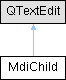
\includegraphics[height=2.000000cm]{class_mdi_child}
\end{center}
\end{figure}
\doxysubsubsection*{Public Member Functions}
\begin{DoxyCompactItemize}
\item 
\Hypertarget{class_mdi_child_acd68748d377124161a52c1a2018b910c}\label{class_mdi_child_acd68748d377124161a52c1a2018b910c} 
void {\bfseries new\+File} ()
\item 
\Hypertarget{class_mdi_child_ac668cf07b620f86b3b090aec69b42013}\label{class_mdi_child_ac668cf07b620f86b3b090aec69b42013} 
bool {\bfseries load\+File} (const QString \&file\+Name)
\item 
\Hypertarget{class_mdi_child_a81e5721add00c46b09be73297b699da2}\label{class_mdi_child_a81e5721add00c46b09be73297b699da2} 
bool {\bfseries save} ()
\item 
\Hypertarget{class_mdi_child_a7c4e80e59aedcb94bb778a0359cdd969}\label{class_mdi_child_a7c4e80e59aedcb94bb778a0359cdd969} 
bool {\bfseries save\+As} ()
\item 
\Hypertarget{class_mdi_child_a686b1bffd947062399b1b47f20180685}\label{class_mdi_child_a686b1bffd947062399b1b47f20180685} 
bool {\bfseries save\+File} (const QString \&file\+Name)
\item 
\Hypertarget{class_mdi_child_a090dfb681fcf406e431090d0d05daa7e}\label{class_mdi_child_a090dfb681fcf406e431090d0d05daa7e} 
QString {\bfseries user\+Friendly\+Current\+File} ()
\item 
\Hypertarget{class_mdi_child_af3545990e356937347d478e60847965b}\label{class_mdi_child_af3545990e356937347d478e60847965b} 
QString {\bfseries current\+File} ()
\item 
\Hypertarget{class_mdi_child_ad65e9d818d571cf3d54d3341a8efc229}\label{class_mdi_child_ad65e9d818d571cf3d54d3341a8efc229} 
bool {\bfseries maybe\+Save} ()
\item 
\Hypertarget{class_mdi_child_abe9adcb39adc8990226d484a6c267e69}\label{class_mdi_child_abe9adcb39adc8990226d484a6c267e69} 
void {\bfseries set\+Current\+File} (const QString \&file\+Name)
\item 
\Hypertarget{class_mdi_child_af3e9797b5a410c3c5714239b2825019a}\label{class_mdi_child_af3e9797b5a410c3c5714239b2825019a} 
QString {\bfseries stripped\+Name} (const QString \&full\+File\+Name)
\item 
\Hypertarget{class_mdi_child_ad59b8edf7a52e505ea612573ff29db6a}\label{class_mdi_child_ad59b8edf7a52e505ea612573ff29db6a} 
void {\bfseries insert\+From\+Menu\+Wizard} (const QString \&value)
\end{DoxyCompactItemize}
\doxysubsubsection*{Public Attributes}
\begin{DoxyCompactItemize}
\item 
\Hypertarget{class_mdi_child_adb18292378edab7f876136f0e94f0eff}\label{class_mdi_child_adb18292378edab7f876136f0e94f0eff} 
QString {\bfseries cur\+File}
\item 
\Hypertarget{class_mdi_child_ab014ad282c46f200e960759bc5506d5c}\label{class_mdi_child_ab014ad282c46f200e960759bc5506d5c} 
bool {\bfseries is\+Untitled}
\item 
\Hypertarget{class_mdi_child_a28d368609c24120e18009a3e0d12566d}\label{class_mdi_child_a28d368609c24120e18009a3e0d12566d} 
\mbox{\hyperlink{class_highlighter}{Highlighter}} \texorpdfstring{$\ast$}{*} {\bfseries highlighter}
\end{DoxyCompactItemize}
\doxysubsubsection*{Protected Member Functions}
\begin{DoxyCompactItemize}
\item 
\Hypertarget{class_mdi_child_ad86c95d4640da91e36b8198cd6db197f}\label{class_mdi_child_ad86c95d4640da91e36b8198cd6db197f} 
void {\bfseries close\+Event} (QClose\+Event \texorpdfstring{$\ast$}{*}event)
\end{DoxyCompactItemize}


The documentation for this class was generated from the following files\+:\begin{DoxyCompactItemize}
\item 
namdi.\+h\item 
namdi.\+cpp\end{DoxyCompactItemize}

\hypertarget{classnaapplication}{\subsection{naapplication \-Class \-Reference}
\label{classnaapplication}\index{naapplication@{naapplication}}
}


{\ttfamily \#include $<$naapplication.\-h$>$}

\subsubsection*{\-Signals}
\begin{DoxyCompactItemize}
\item 
void \hyperlink{classnaapplication_a93d863c2e87e2cdfde862c498e7a9569}{file\-To\-Open} (\-Q\-String \&file)
\item 
void \hyperlink{classnaapplication_a6313292b306f210b04127c720533629c}{url\-To\-Open} (\-Q\-String \&url)
\end{DoxyCompactItemize}
\subsubsection*{\-Public \-Member \-Functions}
\begin{DoxyCompactItemize}
\item 
\hyperlink{classnaapplication_acd4769f83f983ced8e1c36857cade294}{naapplication} (int \&argc, char $\ast$$\ast$argv)
\end{DoxyCompactItemize}
\subsubsection*{\-Protected \-Member \-Functions}
\begin{DoxyCompactItemize}
\item 
virtual bool \hyperlink{classnaapplication_a902a074ff245698124dffce9dba0a800}{event} (\-Q\-Event $\ast$)
\end{DoxyCompactItemize}


\subsubsection{\-Detailed \-Description}


\-Definition at line 9 of file naapplication.\-h.



\subsubsection{\-Constructor \& \-Destructor \-Documentation}
\hypertarget{classnaapplication_acd4769f83f983ced8e1c36857cade294}{\index{naapplication@{naapplication}!naapplication@{naapplication}}
\index{naapplication@{naapplication}!naapplication@{naapplication}}
\paragraph[{naapplication}]{\setlength{\rightskip}{0pt plus 5cm}{\bf naapplication\-::naapplication} (
\begin{DoxyParamCaption}
\item[{int \&}]{argc, }
\item[{char $\ast$$\ast$}]{argv}
\end{DoxyParamCaption}
)}}\label{classnaapplication_acd4769f83f983ced8e1c36857cade294}


\-Definition at line 5 of file naapplication.\-cpp.



\subsubsection{\-Member \-Function \-Documentation}
\hypertarget{classnaapplication_a902a074ff245698124dffce9dba0a800}{\index{naapplication@{naapplication}!event@{event}}
\index{event@{event}!naapplication@{naapplication}}
\paragraph[{event}]{\setlength{\rightskip}{0pt plus 5cm}bool {\bf naapplication\-::event} (
\begin{DoxyParamCaption}
\item[{\-Q\-Event $\ast$}]{event}
\end{DoxyParamCaption}
)\hspace{0.3cm}{\ttfamily  \mbox{[}protected, virtual\mbox{]}}}}\label{classnaapplication_a902a074ff245698124dffce9dba0a800}


\-Definition at line 10 of file naapplication.\-cpp.

\hypertarget{classnaapplication_a93d863c2e87e2cdfde862c498e7a9569}{\index{naapplication@{naapplication}!file\-To\-Open@{file\-To\-Open}}
\index{file\-To\-Open@{file\-To\-Open}!naapplication@{naapplication}}
\paragraph[{file\-To\-Open}]{\setlength{\rightskip}{0pt plus 5cm}void {\bf naapplication\-::file\-To\-Open} (
\begin{DoxyParamCaption}
\item[{\-Q\-String \&}]{file}
\end{DoxyParamCaption}
)\hspace{0.3cm}{\ttfamily  \mbox{[}signal\mbox{]}}}}\label{classnaapplication_a93d863c2e87e2cdfde862c498e7a9569}
\hypertarget{classnaapplication_a6313292b306f210b04127c720533629c}{\index{naapplication@{naapplication}!url\-To\-Open@{url\-To\-Open}}
\index{url\-To\-Open@{url\-To\-Open}!naapplication@{naapplication}}
\paragraph[{url\-To\-Open}]{\setlength{\rightskip}{0pt plus 5cm}void {\bf naapplication\-::url\-To\-Open} (
\begin{DoxyParamCaption}
\item[{\-Q\-String \&}]{url}
\end{DoxyParamCaption}
)\hspace{0.3cm}{\ttfamily  \mbox{[}signal\mbox{]}}}}\label{classnaapplication_a6313292b306f210b04127c720533629c}


\-The documentation for this class was generated from the following files\-:\begin{DoxyCompactItemize}
\item 
\hyperlink{naapplication_8h}{naapplication.\-h}\item 
\hyperlink{naapplication_8cpp}{naapplication.\-cpp}\end{DoxyCompactItemize}

\doxysection{NAClef\+Select Class Reference}
\hypertarget{class_n_a_clef_select}{}\label{class_n_a_clef_select}\index{NAClefSelect@{NAClefSelect}}
Inheritance diagram for NAClef\+Select\+:\begin{figure}[H]
\begin{center}
\leavevmode
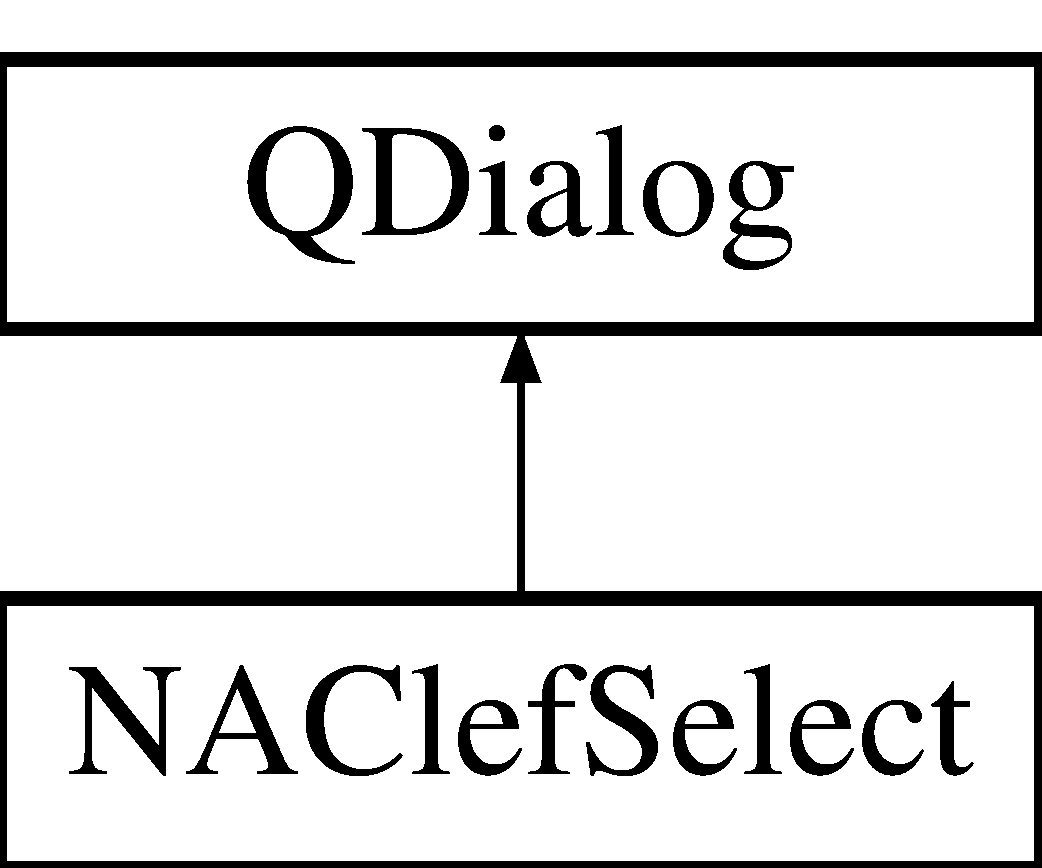
\includegraphics[height=2.000000cm]{class_n_a_clef_select}
\end{center}
\end{figure}
\doxysubsubsection*{Public Member Functions}
\begin{DoxyCompactItemize}
\item 
\Hypertarget{class_n_a_clef_select_ac99b4f68d87cca676886edd849984847}\label{class_n_a_clef_select_ac99b4f68d87cca676886edd849984847} 
{\bfseries NAClef\+Select} (QWidget \texorpdfstring{$\ast$}{*}parent=0)
\end{DoxyCompactItemize}
\doxysubsubsection*{Public Attributes}
\begin{DoxyCompactItemize}
\item 
\Hypertarget{class_n_a_clef_select_a9a1e8ba5db7ac138957613de038783c8}\label{class_n_a_clef_select_a9a1e8ba5db7ac138957613de038783c8} 
QString {\bfseries clefS}
\end{DoxyCompactItemize}


The documentation for this class was generated from the following files\+:\begin{DoxyCompactItemize}
\item 
naclefselect.\+h\item 
naclefselect.\+cpp\end{DoxyCompactItemize}

\hypertarget{classnadoinit}{\subsection{nadoinit \-Class \-Reference}
\label{classnadoinit}\index{nadoinit@{nadoinit}}
}


{\ttfamily \#include $<$nadoinit.\-h$>$}

\subsubsection*{\-Signals}
\begin{DoxyCompactItemize}
\item 
\-Q\-String \hyperlink{classnadoinit_aa9cdbefb183971caf78cd365e26544ed}{path\-Has\-Changed} (\-Q\-String path)
\end{DoxyCompactItemize}
\subsubsection*{\-Public \-Member \-Functions}
\begin{DoxyCompactItemize}
\item 
void \hyperlink{classnadoinit_ade412f43acbc31bfb6a470be1a7655b5}{set\-Values} (\-Q\-String path)
\end{DoxyCompactItemize}
\subsubsection*{\-Public \-Attributes}
\begin{DoxyCompactItemize}
\item 
\-Q\-String\-List \hyperlink{classnadoinit_a69347b16c4be15c8923a6d8785d7af9f}{\-La\-Te\-X\-\_\-\-Path}
\item 
\-Q\-String\-List \hyperlink{classnadoinit_a20f5cafb5bf05df6d89deb43b595a192}{\-Gregorio\-\_\-\-Path}
\item 
\-Q\-String\-List \hyperlink{classnadoinit_a9971fc91456e4cf24927c42471c32e64}{\-Lilypond\-\_\-\-Path}
\item 
\-Q\-String\-List \hyperlink{classnadoinit_a0ea5be240109fb2373f7544bb68a1e4a}{template\-Folder}
\item 
\-Q\-String\-List \hyperlink{classnadoinit_a50b65542641d11f5184a6aa615ba9500}{dict\-Folder}
\item 
\-Q\-String\-List \hyperlink{classnadoinit_a6fd6457d2be15bfa6c13f0d8deba6a08}{help\-Folder}
\item 
\-Q\-String \hyperlink{classnadoinit_a4081a7d29969048e9b81dc07d1421521}{base\-Path}
\item 
\-Q\-String \hyperlink{classnadoinit_a60c7078faeb9e398181107cbd1604ac0}{current\-Path}
\item 
\-Q\-String \hyperlink{classnadoinit_a9a7c2dc3edc0b30cfdb83d2cd8a7b87b}{end\-Text}
\item 
bool \hyperlink{classnadoinit_ac5ebbf07fa035e4dffa8d387ddb22fb7}{isinit}
\end{DoxyCompactItemize}


\subsubsection{\-Detailed \-Description}


\-Definition at line 8 of file nadoinit.\-h.



\subsubsection{\-Member \-Function \-Documentation}
\hypertarget{classnadoinit_aa9cdbefb183971caf78cd365e26544ed}{\index{nadoinit@{nadoinit}!path\-Has\-Changed@{path\-Has\-Changed}}
\index{path\-Has\-Changed@{path\-Has\-Changed}!nadoinit@{nadoinit}}
\paragraph[{path\-Has\-Changed}]{\setlength{\rightskip}{0pt plus 5cm}\-Q\-String {\bf nadoinit\-::path\-Has\-Changed} (
\begin{DoxyParamCaption}
\item[{\-Q\-String}]{path}
\end{DoxyParamCaption}
)\hspace{0.3cm}{\ttfamily  \mbox{[}signal\mbox{]}}}}\label{classnadoinit_aa9cdbefb183971caf78cd365e26544ed}
\hypertarget{classnadoinit_ade412f43acbc31bfb6a470be1a7655b5}{\index{nadoinit@{nadoinit}!set\-Values@{set\-Values}}
\index{set\-Values@{set\-Values}!nadoinit@{nadoinit}}
\paragraph[{set\-Values}]{\setlength{\rightskip}{0pt plus 5cm}void {\bf nadoinit\-::set\-Values} (
\begin{DoxyParamCaption}
\item[{\-Q\-String}]{path}
\end{DoxyParamCaption}
)}}\label{classnadoinit_ade412f43acbc31bfb6a470be1a7655b5}


\subsubsection{\-Member \-Data \-Documentation}
\hypertarget{classnadoinit_a4081a7d29969048e9b81dc07d1421521}{\index{nadoinit@{nadoinit}!base\-Path@{base\-Path}}
\index{base\-Path@{base\-Path}!nadoinit@{nadoinit}}
\paragraph[{base\-Path}]{\setlength{\rightskip}{0pt plus 5cm}\-Q\-String {\bf nadoinit\-::base\-Path}}}\label{classnadoinit_a4081a7d29969048e9b81dc07d1421521}


\-Definition at line 15 of file nadoinit.\-h.

\hypertarget{classnadoinit_a60c7078faeb9e398181107cbd1604ac0}{\index{nadoinit@{nadoinit}!current\-Path@{current\-Path}}
\index{current\-Path@{current\-Path}!nadoinit@{nadoinit}}
\paragraph[{current\-Path}]{\setlength{\rightskip}{0pt plus 5cm}\-Q\-String {\bf nadoinit\-::current\-Path}}}\label{classnadoinit_a60c7078faeb9e398181107cbd1604ac0}


\-Definition at line 15 of file nadoinit.\-h.

\hypertarget{classnadoinit_a50b65542641d11f5184a6aa615ba9500}{\index{nadoinit@{nadoinit}!dict\-Folder@{dict\-Folder}}
\index{dict\-Folder@{dict\-Folder}!nadoinit@{nadoinit}}
\paragraph[{dict\-Folder}]{\setlength{\rightskip}{0pt plus 5cm}\-Q\-String\-List {\bf nadoinit\-::dict\-Folder}}}\label{classnadoinit_a50b65542641d11f5184a6aa615ba9500}


\-Definition at line 14 of file nadoinit.\-h.

\hypertarget{classnadoinit_a9a7c2dc3edc0b30cfdb83d2cd8a7b87b}{\index{nadoinit@{nadoinit}!end\-Text@{end\-Text}}
\index{end\-Text@{end\-Text}!nadoinit@{nadoinit}}
\paragraph[{end\-Text}]{\setlength{\rightskip}{0pt plus 5cm}\-Q\-String {\bf nadoinit\-::end\-Text}}}\label{classnadoinit_a9a7c2dc3edc0b30cfdb83d2cd8a7b87b}


\-Definition at line 15 of file nadoinit.\-h.

\hypertarget{classnadoinit_a20f5cafb5bf05df6d89deb43b595a192}{\index{nadoinit@{nadoinit}!\-Gregorio\-\_\-\-Path@{\-Gregorio\-\_\-\-Path}}
\index{\-Gregorio\-\_\-\-Path@{\-Gregorio\-\_\-\-Path}!nadoinit@{nadoinit}}
\paragraph[{\-Gregorio\-\_\-\-Path}]{\setlength{\rightskip}{0pt plus 5cm}\-Q\-String\-List {\bf nadoinit\-::\-Gregorio\-\_\-\-Path}}}\label{classnadoinit_a20f5cafb5bf05df6d89deb43b595a192}


\-Definition at line 14 of file nadoinit.\-h.

\hypertarget{classnadoinit_a6fd6457d2be15bfa6c13f0d8deba6a08}{\index{nadoinit@{nadoinit}!help\-Folder@{help\-Folder}}
\index{help\-Folder@{help\-Folder}!nadoinit@{nadoinit}}
\paragraph[{help\-Folder}]{\setlength{\rightskip}{0pt plus 5cm}\-Q\-String\-List {\bf nadoinit\-::help\-Folder}}}\label{classnadoinit_a6fd6457d2be15bfa6c13f0d8deba6a08}


\-Definition at line 14 of file nadoinit.\-h.

\hypertarget{classnadoinit_ac5ebbf07fa035e4dffa8d387ddb22fb7}{\index{nadoinit@{nadoinit}!isinit@{isinit}}
\index{isinit@{isinit}!nadoinit@{nadoinit}}
\paragraph[{isinit}]{\setlength{\rightskip}{0pt plus 5cm}bool {\bf nadoinit\-::isinit}}}\label{classnadoinit_ac5ebbf07fa035e4dffa8d387ddb22fb7}


\-Definition at line 16 of file nadoinit.\-h.

\hypertarget{classnadoinit_a69347b16c4be15c8923a6d8785d7af9f}{\index{nadoinit@{nadoinit}!\-La\-Te\-X\-\_\-\-Path@{\-La\-Te\-X\-\_\-\-Path}}
\index{\-La\-Te\-X\-\_\-\-Path@{\-La\-Te\-X\-\_\-\-Path}!nadoinit@{nadoinit}}
\paragraph[{\-La\-Te\-X\-\_\-\-Path}]{\setlength{\rightskip}{0pt plus 5cm}\-Q\-String\-List {\bf nadoinit\-::\-La\-Te\-X\-\_\-\-Path}}}\label{classnadoinit_a69347b16c4be15c8923a6d8785d7af9f}


\-Definition at line 14 of file nadoinit.\-h.

\hypertarget{classnadoinit_a9971fc91456e4cf24927c42471c32e64}{\index{nadoinit@{nadoinit}!\-Lilypond\-\_\-\-Path@{\-Lilypond\-\_\-\-Path}}
\index{\-Lilypond\-\_\-\-Path@{\-Lilypond\-\_\-\-Path}!nadoinit@{nadoinit}}
\paragraph[{\-Lilypond\-\_\-\-Path}]{\setlength{\rightskip}{0pt plus 5cm}\-Q\-String\-List {\bf nadoinit\-::\-Lilypond\-\_\-\-Path}}}\label{classnadoinit_a9971fc91456e4cf24927c42471c32e64}


\-Definition at line 14 of file nadoinit.\-h.

\hypertarget{classnadoinit_a0ea5be240109fb2373f7544bb68a1e4a}{\index{nadoinit@{nadoinit}!template\-Folder@{template\-Folder}}
\index{template\-Folder@{template\-Folder}!nadoinit@{nadoinit}}
\paragraph[{template\-Folder}]{\setlength{\rightskip}{0pt plus 5cm}\-Q\-String\-List {\bf nadoinit\-::template\-Folder}}}\label{classnadoinit_a0ea5be240109fb2373f7544bb68a1e4a}


\-Definition at line 14 of file nadoinit.\-h.



\-The documentation for this class was generated from the following files\-:\begin{DoxyCompactItemize}
\item 
\hyperlink{nadoinit_8h}{nadoinit.\-h}\item 
\hyperlink{nadoinit_8cpp}{nadoinit.\-cpp}\end{DoxyCompactItemize}

\doxysection{NAHeader\+Wizard Class Reference}
\hypertarget{class_n_a_header_wizard}{}\label{class_n_a_header_wizard}\index{NAHeaderWizard@{NAHeaderWizard}}
Inheritance diagram for NAHeader\+Wizard\+:\begin{figure}[H]
\begin{center}
\leavevmode
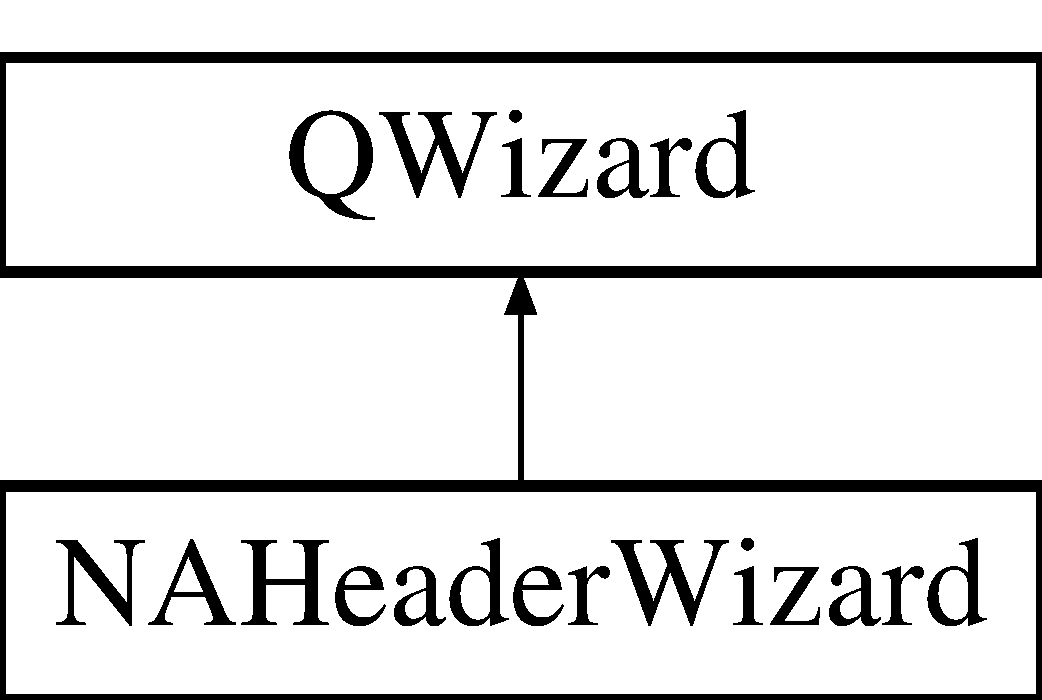
\includegraphics[height=2.000000cm]{class_n_a_header_wizard}
\end{center}
\end{figure}
\doxysubsubsection*{Public Member Functions}
\begin{DoxyCompactItemize}
\item 
\Hypertarget{class_n_a_header_wizard_a0dbd760baa01211319d8862bd68d5517}\label{class_n_a_header_wizard_a0dbd760baa01211319d8862bd68d5517} 
{\bfseries NAHeader\+Wizard} (QWidget \texorpdfstring{$\ast$}{*}parent=0)
\end{DoxyCompactItemize}
\doxysubsubsection*{Public Attributes}
\begin{DoxyCompactItemize}
\item 
\Hypertarget{class_n_a_header_wizard_a911146f3d2b0393517943e7312b0d24e}\label{class_n_a_header_wizard_a911146f3d2b0393517943e7312b0d24e} 
QString\+List {\bfseries header}
\end{DoxyCompactItemize}


The documentation for this class was generated from the following files\+:\begin{DoxyCompactItemize}
\item 
naheaderwizard.\+h\item 
naheaderwizard.\+cpp\end{DoxyCompactItemize}

\hypertarget{class_n_a_help}{\subsection{\-N\-A\-Help \-Class \-Reference}
\label{class_n_a_help}\index{\-N\-A\-Help@{\-N\-A\-Help}}
}


{\ttfamily \#include $<$nahelp.\-h$>$}

\subsubsection*{\-Public \-Member \-Functions}
\begin{DoxyCompactItemize}
\item 
\hyperlink{class_n_a_help_a6f863a832299e25641bf203704f982d3}{\-N\-A\-Help} (\-Q\-Widget $\ast$parent=0)
\item 
\hyperlink{class_n_a_help_a0b0aca837c779a7b1e890c5aa18ba138}{$\sim$\-N\-A\-Help} ()
\item 
void \hyperlink{class_n_a_help_a28861d1e70b5f6fabff9492ef98bf501}{create\-Widgets} ()
\end{DoxyCompactItemize}


\subsubsection{\-Detailed \-Description}


\-Definition at line 18 of file nahelp.\-h.



\subsubsection{\-Constructor \& \-Destructor \-Documentation}
\hypertarget{class_n_a_help_a6f863a832299e25641bf203704f982d3}{\index{\-N\-A\-Help@{\-N\-A\-Help}!\-N\-A\-Help@{\-N\-A\-Help}}
\index{\-N\-A\-Help@{\-N\-A\-Help}!NAHelp@{\-N\-A\-Help}}
\paragraph[{\-N\-A\-Help}]{\setlength{\rightskip}{0pt plus 5cm}{\bf \-N\-A\-Help\-::\-N\-A\-Help} (
\begin{DoxyParamCaption}
\item[{\-Q\-Widget $\ast$}]{parent = {\ttfamily 0}}
\end{DoxyParamCaption}
)\hspace{0.3cm}{\ttfamily  \mbox{[}explicit\mbox{]}}}}\label{class_n_a_help_a6f863a832299e25641bf203704f982d3}


\-Definition at line 5 of file nahelp.\-cpp.

\hypertarget{class_n_a_help_a0b0aca837c779a7b1e890c5aa18ba138}{\index{\-N\-A\-Help@{\-N\-A\-Help}!$\sim$\-N\-A\-Help@{$\sim$\-N\-A\-Help}}
\index{$\sim$\-N\-A\-Help@{$\sim$\-N\-A\-Help}!NAHelp@{\-N\-A\-Help}}
\paragraph[{$\sim$\-N\-A\-Help}]{\setlength{\rightskip}{0pt plus 5cm}{\bf \-N\-A\-Help\-::$\sim$\-N\-A\-Help} (
\begin{DoxyParamCaption}
{}
\end{DoxyParamCaption}
)}}\label{class_n_a_help_a0b0aca837c779a7b1e890c5aa18ba138}


\-Definition at line 14 of file nahelp.\-cpp.



\subsubsection{\-Member \-Function \-Documentation}
\hypertarget{class_n_a_help_a28861d1e70b5f6fabff9492ef98bf501}{\index{\-N\-A\-Help@{\-N\-A\-Help}!create\-Widgets@{create\-Widgets}}
\index{create\-Widgets@{create\-Widgets}!NAHelp@{\-N\-A\-Help}}
\paragraph[{create\-Widgets}]{\setlength{\rightskip}{0pt plus 5cm}void {\bf \-N\-A\-Help\-::create\-Widgets} (
\begin{DoxyParamCaption}
{}
\end{DoxyParamCaption}
)}}\label{class_n_a_help_a28861d1e70b5f6fabff9492ef98bf501}


\-Definition at line 19 of file nahelp.\-cpp.



\-The documentation for this class was generated from the following files\-:\begin{DoxyCompactItemize}
\item 
\hyperlink{nahelp_8h}{nahelp.\-h}\item 
\hyperlink{nahelp_8cpp}{nahelp.\-cpp}\end{DoxyCompactItemize}

\doxysection{nainit Class Reference}
\hypertarget{classnainit}{}\label{classnainit}\index{nainit@{nainit}}
Inheritance diagram for nainit\+:\begin{figure}[H]
\begin{center}
\leavevmode
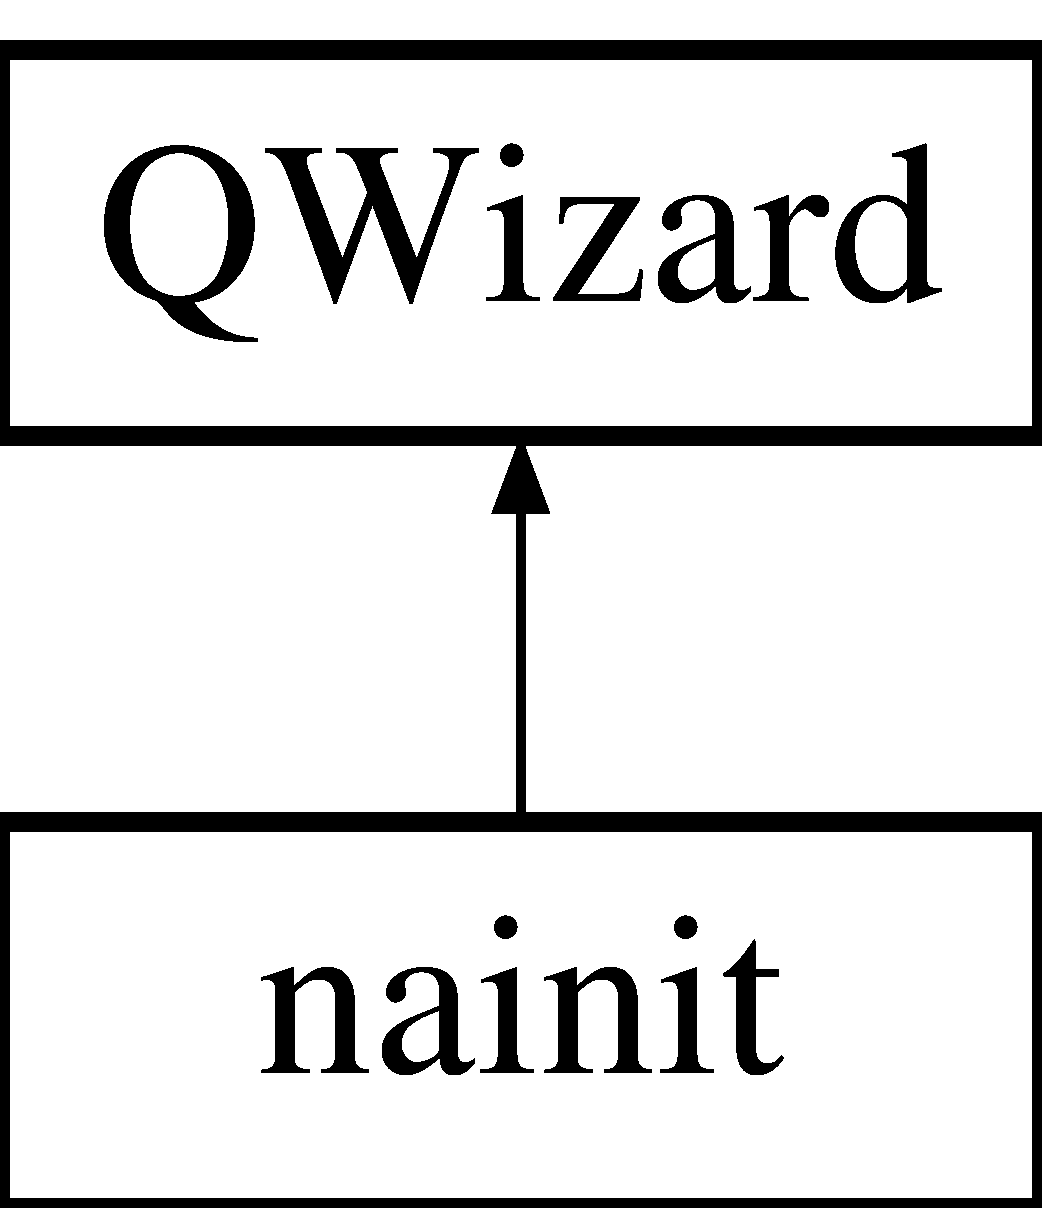
\includegraphics[height=2.000000cm]{classnainit}
\end{center}
\end{figure}
\doxysubsubsection*{Public Slots}
\begin{DoxyCompactItemize}
\item 
\Hypertarget{classnainit_a70db2eca15f8f578ca1bdfd61f084426}\label{classnainit_a70db2eca15f8f578ca1bdfd61f084426} 
void {\bfseries get\+Path} (QString path)
\end{DoxyCompactItemize}
\doxysubsubsection*{Public Member Functions}
\begin{DoxyCompactItemize}
\item 
\Hypertarget{classnainit_aae879af8a4afedb52bedca7064b992e2}\label{classnainit_aae879af8a4afedb52bedca7064b992e2} 
{\bfseries nainit} (QWidget \texorpdfstring{$\ast$}{*}parent=0)
\end{DoxyCompactItemize}
\doxysubsubsection*{Public Attributes}
\begin{DoxyCompactItemize}
\item 
\Hypertarget{classnainit_ad2ef0911b6857edc61203af7fd2d4735}\label{classnainit_ad2ef0911b6857edc61203af7fd2d4735} 
\mbox{\hyperlink{classnadoinit}{nadoinit}} {\bfseries doinit}
\item 
\Hypertarget{classnainit_a719de58a2d8b73e49ad9aacfc389a883}\label{classnainit_a719de58a2d8b73e49ad9aacfc389a883} 
QString {\bfseries La\+Te\+X\+\_\+\+Path}
\item 
\Hypertarget{classnainit_a96612aa4dbefd825d767f626dca65785}\label{classnainit_a96612aa4dbefd825d767f626dca65785} 
QString {\bfseries Gregorio\+\_\+\+Path}
\item 
\Hypertarget{classnainit_a1b91a9100804375dd43cc151f3797c18}\label{classnainit_a1b91a9100804375dd43cc151f3797c18} 
QString {\bfseries Lilypond\+\_\+\+Path}
\item 
\Hypertarget{classnainit_adb261cbd281eaf1341ebea0eadcb0533}\label{classnainit_adb261cbd281eaf1341ebea0eadcb0533} 
QString {\bfseries template\+Folder}
\item 
\Hypertarget{classnainit_a5a80fe813823537dffe5a5975047a597}\label{classnainit_a5a80fe813823537dffe5a5975047a597} 
QString {\bfseries dict\+Folder}
\item 
\Hypertarget{classnainit_a750b8d0712f59b41c1c8b5556b7192b0}\label{classnainit_a750b8d0712f59b41c1c8b5556b7192b0} 
QString {\bfseries help\+Folder}
\end{DoxyCompactItemize}


The documentation for this class was generated from the following files\+:\begin{DoxyCompactItemize}
\item 
nainit.\+h\item 
nainit.\+cpp\end{DoxyCompactItemize}

\doxysection{Na\+Prog Class Reference}
\hypertarget{class_na_prog}{}\label{class_na_prog}\index{NaProg@{NaProg}}
Inheritance diagram for Na\+Prog\+:\begin{figure}[H]
\begin{center}
\leavevmode
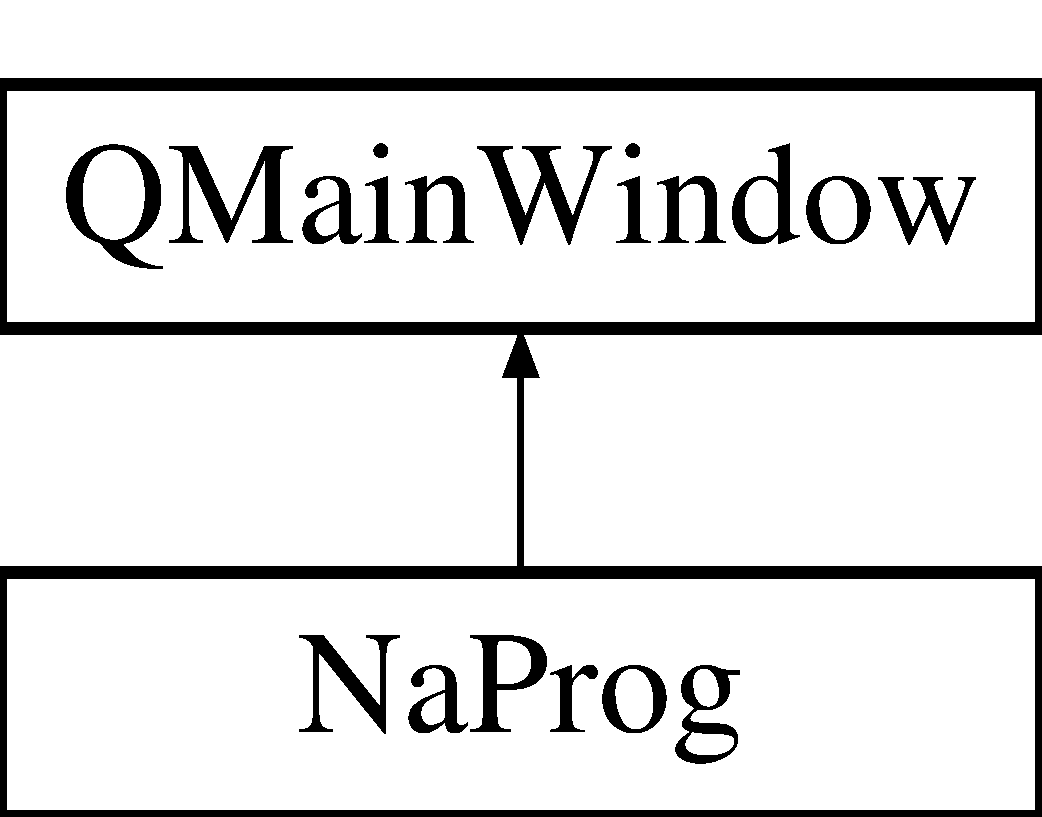
\includegraphics[height=2.000000cm]{class_na_prog}
\end{center}
\end{figure}
\doxysubsubsection*{Public Member Functions}
\begin{DoxyCompactItemize}
\item 
\Hypertarget{class_na_prog_ab7b9d68e5c140356a3d2cf5500cba5f9}\label{class_na_prog_ab7b9d68e5c140356a3d2cf5500cba5f9} 
{\bfseries Na\+Prog} (QWidget \texorpdfstring{$\ast$}{*}parent=0)
\end{DoxyCompactItemize}
\doxysubsubsection*{Public Attributes}
\begin{DoxyCompactItemize}
\item 
\Hypertarget{class_na_prog_a6513c9703c127cd248c8356fbc56d5aa}\label{class_na_prog_a6513c9703c127cd248c8356fbc56d5aa} 
\mbox{\hyperlink{struct_q_header_info}{QHeader\+Info}} {\bfseries hi}
\item 
\Hypertarget{class_na_prog_a082b56ddf4a1e43447690f1dbed98eba}\label{class_na_prog_a082b56ddf4a1e43447690f1dbed98eba} 
QProcess \texorpdfstring{$\ast$}{*} {\bfseries exec\+Prog}
\item 
\Hypertarget{class_na_prog_accbb8cf36587599f0590094829f579cc}\label{class_na_prog_accbb8cf36587599f0590094829f579cc} 
QString {\bfseries La\+Te\+X\+\_\+\+Path}
\item 
\Hypertarget{class_na_prog_a8b2b7aa1b7453a137642cf65fbc3aa8f}\label{class_na_prog_a8b2b7aa1b7453a137642cf65fbc3aa8f} 
QString {\bfseries Lilypond\+\_\+\+Path}
\item 
\Hypertarget{class_na_prog_adcfd69f235ef30aadf54d95bc5ea30e4}\label{class_na_prog_adcfd69f235ef30aadf54d95bc5ea30e4} 
QString {\bfseries Gregorio\+\_\+\+Path}
\item 
\Hypertarget{class_na_prog_a0fcce578ce90177d45025fbdd052cbbf}\label{class_na_prog_a0fcce578ce90177d45025fbdd052cbbf} 
QString {\bfseries tmpl\+Name}
\item 
\Hypertarget{class_na_prog_a32ab16fb09891c4ceff345c8231f71b2}\label{class_na_prog_a32ab16fb09891c4ceff345c8231f71b2} 
QString {\bfseries template\+Folder}
\item 
\Hypertarget{class_na_prog_a356f2ad14ea8b3f248af4bf1ae055246}\label{class_na_prog_a356f2ad14ea8b3f248af4bf1ae055246} 
QString {\bfseries dict\+Folder}
\end{DoxyCompactItemize}
\doxysubsubsection*{Protected Member Functions}
\begin{DoxyCompactItemize}
\item 
\Hypertarget{class_na_prog_a362e8434f30ec3c51d9262653e07b83a}\label{class_na_prog_a362e8434f30ec3c51d9262653e07b83a} 
void {\bfseries change\+Event} (QEvent \texorpdfstring{$\ast$}{*}e)
\end{DoxyCompactItemize}


The documentation for this class was generated from the following files\+:\begin{DoxyCompactItemize}
\item 
naprog.\+h\item 
naprog.\+cpp\end{DoxyCompactItemize}

\doxysection{napsalm Class Reference}
\hypertarget{classnapsalm}{}\label{classnapsalm}\index{napsalm@{napsalm}}


Class for holding the information on psalm tone models.  




{\ttfamily \#include $<$napsalm.\+h$>$}



\doxysubsection{Detailed Description}
Class for holding the information on psalm tone models. 

The documentation for this class was generated from the following file\+:\begin{DoxyCompactItemize}
\item 
napsalm.\+h\end{DoxyCompactItemize}

\doxysection{NASettings Class Reference}
\hypertarget{class_n_a_settings}{}\label{class_n_a_settings}\index{NASettings@{NASettings}}


Settings class, holds some variables for the settings dialog and the dialog itself.  


Inheritance diagram for NASettings\+:\begin{figure}[H]
\begin{center}
\leavevmode
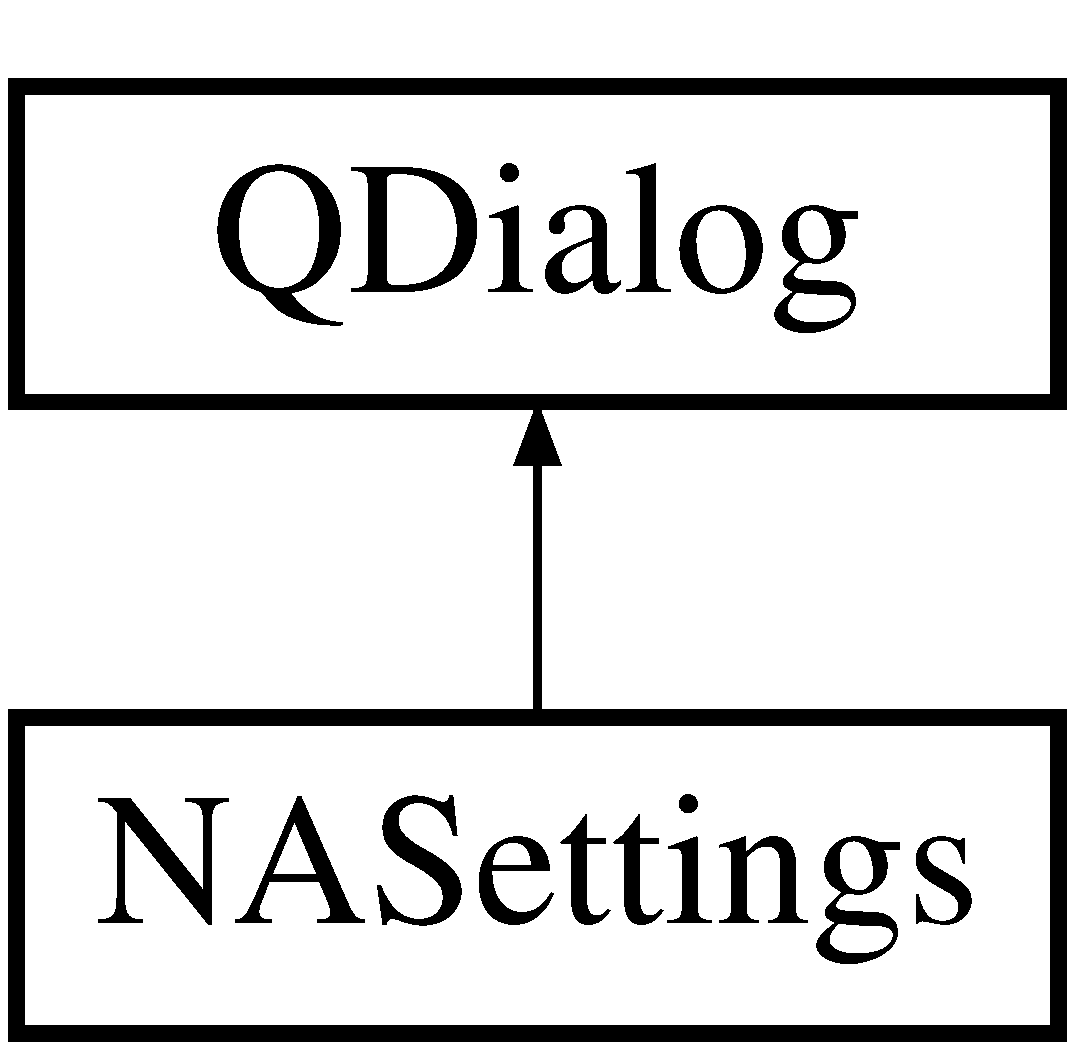
\includegraphics[height=2.000000cm]{class_n_a_settings}
\end{center}
\end{figure}
\doxysubsubsection*{Public Member Functions}
\begin{DoxyCompactItemize}
\item 
\Hypertarget{class_n_a_settings_a800fd08e1ce3ebb92cfaa3ab06383018}\label{class_n_a_settings_a800fd08e1ce3ebb92cfaa3ab06383018} 
{\bfseries NASettings} (QWidget \texorpdfstring{$\ast$}{*}parent=0)
\end{DoxyCompactItemize}
\doxysubsubsection*{Public Attributes}
\begin{DoxyCompactItemize}
\item 
\Hypertarget{class_n_a_settings_a350ad35ee9f5f7b281dc737c856c60b6}\label{class_n_a_settings_a350ad35ee9f5f7b281dc737c856c60b6} 
QColor {\bfseries keyword}
\item 
\Hypertarget{class_n_a_settings_a5664018dde5193a8f5e16c52fb0caf48}\label{class_n_a_settings_a5664018dde5193a8f5e16c52fb0caf48} 
QColor {\bfseries commentary}
\item 
\Hypertarget{class_n_a_settings_af6987962f1746780b2f33ffb370498c0}\label{class_n_a_settings_af6987962f1746780b2f33ffb370498c0} 
QColor {\bfseries pitch}
\item 
\Hypertarget{class_n_a_settings_a87da2bfd4a25e0eafde61fb41c9a4931}\label{class_n_a_settings_a87da2bfd4a25e0eafde61fb41c9a4931} 
QColor {\bfseries translation}
\item 
\Hypertarget{class_n_a_settings_ada0b15c317a1902885d9719a24a071b6}\label{class_n_a_settings_ada0b15c317a1902885d9719a24a071b6} 
QString {\bfseries fontsize}
\item 
\Hypertarget{class_n_a_settings_aa0fd38ef4993f6982c3147642912572a}\label{class_n_a_settings_aa0fd38ef4993f6982c3147642912572a} 
QString {\bfseries staffsize}
\end{DoxyCompactItemize}
\doxysubsubsection*{Protected Member Functions}
\begin{DoxyCompactItemize}
\item 
\Hypertarget{class_n_a_settings_a4b5e6d70064378bd3a5d5a9789322208}\label{class_n_a_settings_a4b5e6d70064378bd3a5d5a9789322208} 
void {\bfseries change\+Event} (QEvent \texorpdfstring{$\ast$}{*}e)
\end{DoxyCompactItemize}


\doxysubsection{Detailed Description}
Settings class, holds some variables for the settings dialog and the dialog itself. 

The documentation for this class was generated from the following files\+:\begin{DoxyCompactItemize}
\item 
nasettings.\+h\item 
nasettings.\+cpp\end{DoxyCompactItemize}

\input{class_na_view}
\doxysection{QHeader\+Info Struct Reference}
\hypertarget{struct_q_header_info}{}\label{struct_q_header_info}\index{QHeaderInfo@{QHeaderInfo}}
\doxysubsubsection*{Public Attributes}
\begin{DoxyCompactItemize}
\item 
\Hypertarget{struct_q_header_info_a3bb30548b15d8eef6f3db0feab710547}\label{struct_q_header_info_a3bb30548b15d8eef6f3db0feab710547} 
QString {\bfseries name}
\begin{DoxyCompactList}\small\item\em \doxylink{struct_q_header_info}{QHeader\+Info} holds the parts of the GABC file header. \end{DoxyCompactList}\item 
\Hypertarget{struct_q_header_info_aa22ae31b6e02a706caa264837a74b0f1}\label{struct_q_header_info_aa22ae31b6e02a706caa264837a74b0f1} 
QString {\bfseries arranger}
\item 
\Hypertarget{struct_q_header_info_a2be3aad33898ebedc8867632f97df59f}\label{struct_q_header_info_a2be3aad33898ebedc8867632f97df59f} 
QString {\bfseries officepart}
\item 
\Hypertarget{struct_q_header_info_a0f1252cbbf70ea7922af484c4d722221}\label{struct_q_header_info_a0f1252cbbf70ea7922af484c4d722221} 
QString {\bfseries mode}
\item 
\Hypertarget{struct_q_header_info_aef733de4162356858613ae27e6d7613a}\label{struct_q_header_info_aef733de4162356858613ae27e6d7613a} 
QString {\bfseries annotation1}
\item 
\Hypertarget{struct_q_header_info_a8840a0de86eed80a0f069b561beab4f0}\label{struct_q_header_info_a8840a0de86eed80a0f069b561beab4f0} 
QString {\bfseries annotation2}
\item 
\Hypertarget{struct_q_header_info_a7e11b1cd2cce125b9ed883c2c0012565}\label{struct_q_header_info_a7e11b1cd2cce125b9ed883c2c0012565} 
QString {\bfseries commentary}
\item 
\Hypertarget{struct_q_header_info_ac2259a058ed33551fac5b902e6e37cf6}\label{struct_q_header_info_ac2259a058ed33551fac5b902e6e37cf6} 
QString {\bfseries font}
\item 
\Hypertarget{struct_q_header_info_a2826d9a8b24977f47136c6f686688927}\label{struct_q_header_info_a2826d9a8b24977f47136c6f686688927} 
QString {\bfseries gabccopy}
\item 
\Hypertarget{struct_q_header_info_abbc732261ea771cae1a9b28e6832e947}\label{struct_q_header_info_abbc732261ea771cae1a9b28e6832e947} 
QString {\bfseries scorecopy}
\item 
\Hypertarget{struct_q_header_info_a31870c13a97c9b45b42a072e5ac516e2}\label{struct_q_header_info_a31870c13a97c9b45b42a072e5ac516e2} 
QString {\bfseries occasion}
\item 
\Hypertarget{struct_q_header_info_acfabb4e5b787c1fb3aadf3fa422ec363}\label{struct_q_header_info_acfabb4e5b787c1fb3aadf3fa422ec363} 
QString {\bfseries meter}
\item 
\Hypertarget{struct_q_header_info_aeaa183023b432322b3ebd3c9e4d55ec2}\label{struct_q_header_info_aeaa183023b432322b3ebd3c9e4d55ec2} 
QString {\bfseries author}
\item 
\Hypertarget{struct_q_header_info_ab5493aa10e4dc6cfd8e99b8d426dcd6b}\label{struct_q_header_info_ab5493aa10e4dc6cfd8e99b8d426dcd6b} 
QString {\bfseries date}
\item 
\Hypertarget{struct_q_header_info_af3f5666b4bb13ca460a8f593b82e5ac1}\label{struct_q_header_info_af3f5666b4bb13ca460a8f593b82e5ac1} 
QString {\bfseries manuscript}
\item 
\Hypertarget{struct_q_header_info_a136a32d2c0ea2da173168909fcee5de9}\label{struct_q_header_info_a136a32d2c0ea2da173168909fcee5de9} 
QString {\bfseries mreference}
\item 
\Hypertarget{struct_q_header_info_ab94be4daad3a5925bac217386ddf5a26}\label{struct_q_header_info_ab94be4daad3a5925bac217386ddf5a26} 
QString {\bfseries book}
\item 
\Hypertarget{struct_q_header_info_a9ab2205d189840873e74b6a324a3e55f}\label{struct_q_header_info_a9ab2205d189840873e74b6a324a3e55f} 
QString {\bfseries transcriber}
\item 
\Hypertarget{struct_q_header_info_af1a107397da7f4586dc81e51792f7784}\label{struct_q_header_info_af1a107397da7f4586dc81e51792f7784} 
QString {\bfseries tdate}
\item 
\Hypertarget{struct_q_header_info_a647735abe52888bdcad120f84926a0fe}\label{struct_q_header_info_a647735abe52888bdcad120f84926a0fe} 
QString {\bfseries instyle}
\item 
\Hypertarget{struct_q_header_info_ae964c403b750706da770391ec91bf2fd}\label{struct_q_header_info_ae964c403b750706da770391ec91bf2fd} 
QString {\bfseries notes}
\end{DoxyCompactItemize}


The documentation for this struct was generated from the following file\+:\begin{DoxyCompactItemize}
\item 
naprog.\+h\end{DoxyCompactItemize}

\doxysection{QHelp\+Browser Class Reference}
\hypertarget{class_q_help_browser}{}\label{class_q_help_browser}\index{QHelpBrowser@{QHelpBrowser}}
Inheritance diagram for QHelp\+Browser\+:\begin{figure}[H]
\begin{center}
\leavevmode
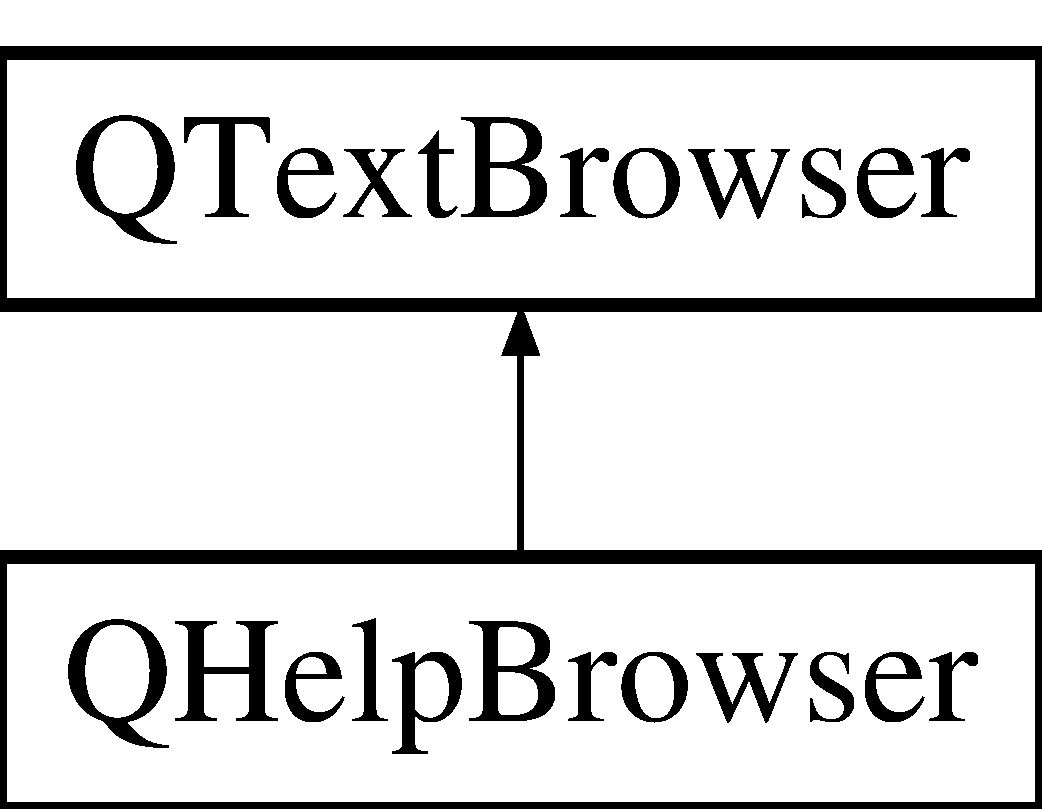
\includegraphics[height=2.000000cm]{class_q_help_browser}
\end{center}
\end{figure}
\doxysubsubsection*{Public Member Functions}
\begin{DoxyCompactItemize}
\item 
\Hypertarget{class_q_help_browser_a84614ea262e0c8816b0294d072b2445a}\label{class_q_help_browser_a84614ea262e0c8816b0294d072b2445a} 
{\bfseries QHelp\+Browser} (QString collection\+File, QWidget \texorpdfstring{$\ast$}{*}parent)
\item 
\Hypertarget{class_q_help_browser_aacffe80832bb6258bcca12aa55548d23}\label{class_q_help_browser_aacffe80832bb6258bcca12aa55548d23} 
void {\bfseries show\+Help\+For\+Keyword} (const QString \&id)
\end{DoxyCompactItemize}


The documentation for this class was generated from the following files\+:\begin{DoxyCompactItemize}
\item 
nahelp.\+h\item 
nahelp.\+cpp\end{DoxyCompactItemize}

\section{\-File \-Documentation}
\hypertarget{hnjalloc_8c}{\subsection{hnjalloc.\-c \-File \-Reference}
\label{hnjalloc_8c}\index{hnjalloc.\-c@{hnjalloc.\-c}}
}
{\ttfamily \#include $<$stdlib.\-h$>$}\*
{\ttfamily \#include $<$stdio.\-h$>$}\*
\subsubsection*{\-Functions}
\begin{DoxyCompactItemize}
\item 
void $\ast$ \hyperlink{hnjalloc_8c_ace86d15506925c7cf93c03c4cd99d5b0}{hnj\-\_\-malloc} (int size)
\item 
void $\ast$ \hyperlink{hnjalloc_8c_ac97a4540e1a0adbb94bdf3340d74c6a0}{hnj\-\_\-realloc} (void $\ast$p, int size)
\item 
void \hyperlink{hnjalloc_8c_a67f30821d3081d04984d0009d2a41aa9}{hnj\-\_\-free} (void $\ast$p)
\end{DoxyCompactItemize}


\subsubsection{\-Function \-Documentation}
\hypertarget{hnjalloc_8c_a67f30821d3081d04984d0009d2a41aa9}{\index{hnjalloc.\-c@{hnjalloc.\-c}!hnj\-\_\-free@{hnj\-\_\-free}}
\index{hnj\-\_\-free@{hnj\-\_\-free}!hnjalloc.c@{hnjalloc.\-c}}
\paragraph[{hnj\-\_\-free}]{\setlength{\rightskip}{0pt plus 5cm}void {\bf hnj\-\_\-free} (
\begin{DoxyParamCaption}
\item[{void $\ast$}]{p}
\end{DoxyParamCaption}
)}}\label{hnjalloc_8c_a67f30821d3081d04984d0009d2a41aa9}


\-Definition at line 68 of file hnjalloc.\-c.

\hypertarget{hnjalloc_8c_ace86d15506925c7cf93c03c4cd99d5b0}{\index{hnjalloc.\-c@{hnjalloc.\-c}!hnj\-\_\-malloc@{hnj\-\_\-malloc}}
\index{hnj\-\_\-malloc@{hnj\-\_\-malloc}!hnjalloc.c@{hnjalloc.\-c}}
\paragraph[{hnj\-\_\-malloc}]{\setlength{\rightskip}{0pt plus 5cm}void$\ast$ {\bf hnj\-\_\-malloc} (
\begin{DoxyParamCaption}
\item[{int}]{size}
\end{DoxyParamCaption}
)}}\label{hnjalloc_8c_ace86d15506925c7cf93c03c4cd99d5b0}


\-Definition at line 42 of file hnjalloc.\-c.

\hypertarget{hnjalloc_8c_ac97a4540e1a0adbb94bdf3340d74c6a0}{\index{hnjalloc.\-c@{hnjalloc.\-c}!hnj\-\_\-realloc@{hnj\-\_\-realloc}}
\index{hnj\-\_\-realloc@{hnj\-\_\-realloc}!hnjalloc.c@{hnjalloc.\-c}}
\paragraph[{hnj\-\_\-realloc}]{\setlength{\rightskip}{0pt plus 5cm}void$\ast$ {\bf hnj\-\_\-realloc} (
\begin{DoxyParamCaption}
\item[{void $\ast$}]{p, }
\item[{int}]{size}
\end{DoxyParamCaption}
)}}\label{hnjalloc_8c_ac97a4540e1a0adbb94bdf3340d74c6a0}


\-Definition at line 56 of file hnjalloc.\-c.


\input{hnjalloc_8h}
\input{hyphen_8c}
\input{hyphen_8h}
\input{main_8cpp}
\input{naapplication_8cpp}
\hypertarget{naapplication_8h}{\subsection{naapplication.\-h \-File \-Reference}
\label{naapplication_8h}\index{naapplication.\-h@{naapplication.\-h}}
}
{\ttfamily \#include $<$\-Q\-Application$>$}\*
{\ttfamily \#include $<$\-Q\-String$>$}\*
{\ttfamily \#include $<$\-Q\-File\-Open\-Event$>$}\*
{\ttfamily \#include $<$\-Q\-Url$>$}\*
\subsubsection*{\-Classes}
\begin{DoxyCompactItemize}
\item 
class \hyperlink{classnaapplication}{naapplication}
\end{DoxyCompactItemize}

\hypertarget{naclefselect_8cpp}{\subsection{naclefselect.\-cpp \-File \-Reference}
\label{naclefselect_8cpp}\index{naclefselect.\-cpp@{naclefselect.\-cpp}}
}
{\ttfamily \#include \char`\"{}naclefselect.\-h\char`\"{}}\*
{\ttfamily \#include \char`\"{}ui\-\_\-naclefselect.\-h\char`\"{}}\*

\hypertarget{naclefselect_8h}{\subsection{naclefselect.\-h \-File \-Reference}
\label{naclefselect_8h}\index{naclefselect.\-h@{naclefselect.\-h}}
}
{\ttfamily \#include $<$\-Q\-Dialog$>$}\*
\subsubsection*{\-Classes}
\begin{DoxyCompactItemize}
\item 
class \hyperlink{class_n_a_clef_select}{\-N\-A\-Clef\-Select}
\end{DoxyCompactItemize}
\subsubsection*{\-Namespaces}
\begin{DoxyCompactItemize}
\item 
namespace \hyperlink{namespace_ui}{\-Ui}
\end{DoxyCompactItemize}

\input{nadoinit_8cpp}
\input{nadoinit_8h}
\hypertarget{naheaderwizard_8cpp}{\subsection{naheaderwizard.\-cpp \-File \-Reference}
\label{naheaderwizard_8cpp}\index{naheaderwizard.\-cpp@{naheaderwizard.\-cpp}}
}
{\ttfamily \#include \char`\"{}naheaderwizard.\-h\char`\"{}}\*
{\ttfamily \#include \char`\"{}ui\-\_\-naheaderwizard.\-h\char`\"{}}\*

\input{naheaderwizard_8h}
\hypertarget{nahelp_8cpp}{\subsection{nahelp.\-cpp \-File \-Reference}
\label{nahelp_8cpp}\index{nahelp.\-cpp@{nahelp.\-cpp}}
}
{\ttfamily \#include \char`\"{}nahelp.\-h\char`\"{}}\*
{\ttfamily \#include \char`\"{}ui\-\_\-nahelp.\-h\char`\"{}}\*
{\ttfamily \#include $<$\-Q\-Message\-Box$>$}\*

\input{nahelp_8h}
\hypertarget{nainit_8cpp}{\subsection{nainit.\-cpp \-File \-Reference}
\label{nainit_8cpp}\index{nainit.\-cpp@{nainit.\-cpp}}
}
{\ttfamily \#include \char`\"{}nainit.\-h\char`\"{}}\*
{\ttfamily \#include \char`\"{}ui\-\_\-nainit.\-h\char`\"{}}\*

\hypertarget{nainit_8h}{\subsection{nainit.\-h \-File \-Reference}
\label{nainit_8h}\index{nainit.\-h@{nainit.\-h}}
}
{\ttfamily \#include $<$\-Q\-Wizard$>$}\*
{\ttfamily \#include $<$\-Q\-Text\-Edit$>$}\*
{\ttfamily \#include \char`\"{}ui\-\_\-nainit.\-h\char`\"{}}\*
{\ttfamily \#include \char`\"{}nadoinit.\-h\char`\"{}}\*
\subsubsection*{\-Classes}
\begin{DoxyCompactItemize}
\item 
class \hyperlink{classnainit}{nainit}
\end{DoxyCompactItemize}
\subsubsection*{\-Namespaces}
\begin{DoxyCompactItemize}
\item 
namespace \hyperlink{namespace_ui}{\-Ui}
\end{DoxyCompactItemize}

\input{namdi_8cpp}
\hypertarget{namdi_8h}{\subsection{namdi.\-h \-File \-Reference}
\label{namdi_8h}\index{namdi.\-h@{namdi.\-h}}
}
{\ttfamily \#include $<$\-Q\-Text\-Edit$>$}\*
{\ttfamily \#include $<$\-Q\-Settings$>$}\*
{\ttfamily \#include \char`\"{}nasyntax.\-h\char`\"{}}\*
\subsubsection*{\-Classes}
\begin{DoxyCompactItemize}
\item 
class \hyperlink{class_mdi_child}{\-Mdi\-Child}
\end{DoxyCompactItemize}

\hypertarget{naprog_8cpp}{\subsection{naprog.\-cpp \-File \-Reference}
\label{naprog_8cpp}\index{naprog.\-cpp@{naprog.\-cpp}}
}
{\ttfamily \#include \char`\"{}naprog.\-h\char`\"{}}\*
{\ttfamily \#include \char`\"{}ui\-\_\-naprog.\-h\char`\"{}}\*

\input{naprog_8h}
\input{napsalm_8cpp}
\input{napsalm_8h}
\input{nasettings_8cpp}
\input{nasettings_8h}
\input{nasyntax_8cpp}
\input{nasyntax_8h}
\input{naview_8cpp}
\input{naview_8h}
\input{version_8h}
\printindex
\end{document}
